DNA read mappers have to process a huge number of DNA reads as fast as possible. DNA reads are not related to each other, hence there is no obstacle in processing multiple of them at the same time. The first way to parallelise the mapping is to use multiple CPU threads. BWA-MEM supports multhreading mode where each CPU thread maps one DNA read. But the number of threads on a CPU is often very limited, as a single CPU has at best a few dozen of cores. Other types of hardware can present more parallelism.

To accelerate the computation, several approaches were tried. For example, Ahmed \emph{et al.} used a dedicated FPGA (\emph{Field Programmable Gate Array}) to accelerate the research with the FM-index and the extension~\cite{Ahmed:FPGA}. Another approach from Mashtaq \emph{et al.} consisted in streaming DNA sequences alignment tasks to a cluster with Apache Spark~\cite{Mushtaq:spark}. But these solutions require extra hardware and can be difficult to set up. We would like to propose a solution using common hardware found on computers, in particular, Graphics Processing Units, or GPUs.

%Furthermore, looking into a full genome for a match would be an incredibly tedious task without an efficient search algorithm. It is then advisable to create an index of the reference genome. With this index, operations to research a given pattern in a huge data set can be faster than linear time with respect to the data size.
DNA computation can take advantage of the inner structure of a GPU to compute the alignment faster. The use of GPUs have been investigated for DNA acceleration, first for global alignment~\cite{gpualignglobal}, then in the NVBIO CUDA library~\cite{nvidia:nvbio}, and later for semi-global and local alignment with on-GPU data compression~\cite{Ahmed:gasal}. GPUs have been proven very efficient for these tasks. First, we will quickly review the current solutions at hand. Then a presentation of the GPU architecture and programming paradigm will show how these devices work and how they are adapted for this work.

\subsection{Parallel computing for DNA alignment}
In the seed-extension stage, DNA read mapper align a pair of sequences (pairwise alignment) using a sequence alignment algorithm.
The computation for alignment between two DNA strings is intensive, yet simple. The main problem comes from the input data size. Each DNA reads have many seed hits and each seed have to be extended. Hence, a large number of seed-extension have to be performed. Still, it is important to note that each pairwise alignment is independent from the others. A simple and effective way to accelerate the computation is to parallelise it. On a computer, one can use multiple threads on a CPU to achieve that parallelisation and compute several alignments at the same time. However, the number of threads available on a CPU is limited to a dozen, or a few dozen at best; but Graphics Computing Units (GPUs) can have hundreds to thousands of cores at disposal. This makes GPUs a hardware of choice for acceleration using parallel computing. Running multiple alignments in parallel is called \emph{inter-sequence parallelisation}. 

It is possible to go even further with \emph{intra-sequence parallelisation}, that is, to calculate the dynamic programming matrix with multiple threads. This implies having synchronisation phases: since the cell values depends on the previously calculated ones, it implies processing with a logic order, and require a high level of optimisation for efficient speed-up~\cite{Houtgast:gpu-accelerated}. Although this have many advantages in speed but also in power consumption~\cite{Houtgast:power-efficiency}, they require specific hardware, and we will not explore this topic later on.

As for current solutions, a lot of solutions exist~\cite{wiki:ListAlignmentSoft} so we will only name some of the existing softwares for DNA alignment. These tools are most often present as libraries, to be able to integrate them in bigger and more easy-to-use software.

\begin{itemize}
    \item \emph{SeqAn}~\cite{Doring:seqan} is a C++ toolbox for DNA alignment. It features a lot of various tools, and implements its own C++ library for alignment. It runs on multiple CPU threads, and can rely on SIMD instructions for inter and intra sequence parallelisation. Both AVX2 S as well AVX512 SIMD instruction sets are supported.
    \item \emph{Basic Local Alignment Seach Tool} (\emph{BLAST})~\cite{Altschul:BLAST} searches for pairwise alignment with the seed-extension method,
    \item \emph{Bowtie2}~\cite{Langmead:bowtie} is a fast and lightweight DNA aligner that runs even on low-end machines. It allows for up to two mismatches in the seeding phase and in general it reaches maximum efficiency by trading exactness for reasonable heuristics.
    % BWA is not a generic tool but more like a complete software.
    %\item \emph{Burrows-Wheeler Aligner} (\emph{BWA})~\cite{li:bwa} is a DNA aligner focused on speed relying on FM-index for seeding, with BLAST-like extension,
    \item \emph{NVBIO}~\cite{nvidia:nvbio} is a GPU-accelerated library written in CUDA, the dedicated language for general-purpose GPU computing on NVIDIA GPUs. It has a lot of features including banded dynamic programming, fast FM-index construction, and efficient data handling between CPU and GPU.
    \item \emph{GASAL2}~\cite{Ahmed:gasal2} is also a CUDA-written library for DNA alignment, developed with speed in mind. Despite its relatively small number of features, it runs all compute-intensive parts on GPU for maximum speed-up.
\end{itemize}


\subsection{General-purpose GPU computing basics}

Historically, GPUs have been developed to render graphics, and because of this purpose, have a highly parallel architecture to cope with independent parts of the picture. GPUs can now be used for generic computing, as a separate accelerator towards which the CPU can offload parts of the computation. As such, they have large number of cores, orders of magnitude higher than CPUs (several thousands versus a few dozen). Yet, programming on GPU highly depends on the hardware at hand. There is an open programming framework called \emph{OpenCL}~\cite{misc:opencl} and it has the advantage of being cross-platform for all GPUs and royalty-free; yet it is quite complex to write and run. Hence a lot of people are rather using CUDA~\cite{misc:cuda}, the proprietary framework to program NVIDIA GPUs. For the rest of the thesis, we will only focus on NVIDIA GPU architecture and CUDA.

We introduce the terms \emph{host} to designate the CPU-side of the machine, constituted of the CPU and its RAM; and \emph{device} the GPU-side with its dedicated onboard memory called \emph{global memory} or \emph{VRAM}, short for Video RAM. Figure~\ref{fig:gpu-arch} shows a summarised view of the CPU-GPU tandem. First, the CPU "host" transfers data from the RAM to the device VRAM. Then the CPU launches parallel functions called \emph{kernels} on the GPU. This kernel is launched on a \emph{grid}, divided into \emph{blocks}, each of them having a certain number of \emph{threads}. The grid and block sizes are specified as launch parameters, and they are adapted to divide all the data to process into a suited number of threads. Inside a block, threads can access a shared memory. Scopes from different memories are specified on Figure~\ref{fig:gpu-memory-scope}. Each thread executes an instance of the kernel, has thread ID and has its own private memory for local variables. Threads in a block access a shared memory, allowing to synchronise them and share data. Blocks are arranged in grids, and grids share data with a memory space allocated for the application context in global memory.

\begin{figure}[h]
	\centering
	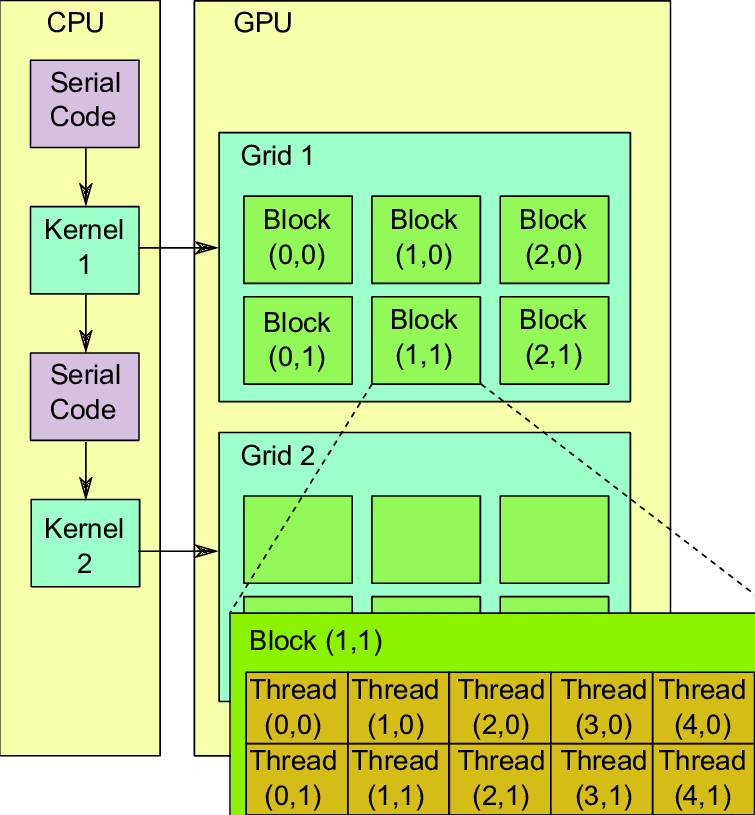
\includegraphics[width=0.6\linewidth]{gpu-arch}
	\caption{GPU architecture schematics (from~\cite{Bartezzaghi:gpu-arch})}
	\label{fig:gpu-arch}
\end{figure}

\begin{figure}[h]
	\centering
	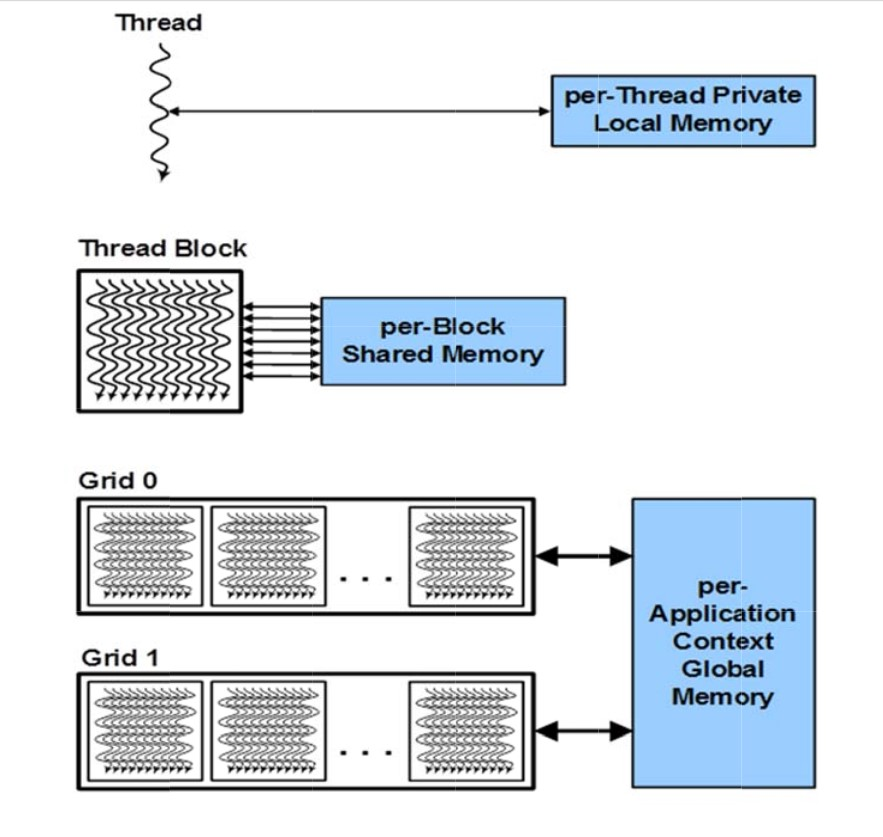
\includegraphics[width=0.6\linewidth]{gpu-memory-scope}
	\caption{GPU memories scope (from~\cite{nvidia:keplerarch})}
	\label{fig:gpu-memory-scope}
\end{figure}

When the computation is done on the GPU, output data is available in VRAM. The CPU can then fetch the results from VRAM to load them in RAM, so that they can be further processed, stored or displayed.

In our case, we use NVIDIA GPUs that present their own particularities in the architecture~\cite{nvidia:keplerarch}. NVIDIA GPUs organise computing resources in Streaming Multiprocessors (SM). We will describe the features from the Kepler architecture since it is the hardware we used for this thesis. For example, the Kepler architecture features 15 SMs which share an L2 cache. Each SM has an instruction cache, L1 cache used as shared memory, texture memories, and a set of computing resources. The main computing core are \emph{CUDA cores} or Stream Processors (SP) for single-precision calculation. But there are also double-precision units, special functions units, and load/store units to manage registry operations. 

%\warn{add picture from Kepler Architecture}

This presents two main benefits. First, some problems that can be highly parallelisable will take advantage of the huge number of GPU cores. Second, being able to offload the calculation to a separate device means that both the CPU and the GPU are busy at the same time: this enables hidden-time computation, that is, the CPU can continue to execute another part of the code while the kernel is running on the GPU runs its part, and the former can retrieve the results only when the latter is done.

Hidden time capability is achieved thanks to non-blocking launches and streams~\cite{misc:cudastreams}. Streams are execution environments for GPUs. For several years now, it is possible to launch multiple threads of the same function on the GPU, the \emph{kernel}, without needing to wait for all kernel instances to finish. The GPU kernel launch returns immediately, and the host can perform other tasks while the kernel is running on the GPU, and the host simply checks if the stream has finished. For example, a program declares two streams, the host can launch the kernel on Stream~\#1, then fill up the data for Stream~\#2 while the first one computes. When Stream~\#2 is launched, by that time, Stream~\#1 has finished, so results can be retrieved and Stream~\#1 can be filled again with the next data to compute while Stream~\#2 computes; and so on. The simple principle is explained here with two streams, but one can use as many streams as needed to utilise the GPU resources as much as possible.

It is crucial to monitor some metrics to ensure the GPU is used to its fullest, and has its own limited resources. We can mention:

\begin{itemize}
	\item occupancy (in \%): it represents how much of the computing resources are used, so the fraction of SP in use when a kernel is running.
	\item VRAM use (in MB): it is the onboard memory and cannot be exceeded.
	\item data transfer time: since it is a separate device, it is important to check if data transfers are taking more or less time than the computation part.
\end{itemize}

\subsection{Motivation}
We have seen that DNA mapping is a time-consuming task and that various techniques have been tried to accelerate it. In particular, parallelisation is a way to reach high throughput by using adequate hardware. However, the approaches tried present a huge drawback for DNA scientists. When they rely on a DNA mapper like BWA-MEM, they expect to trust the output of the tool they work with. Hence, an accelerated BWA-MEM must provide matching results with the original BWA-MEM.

Many of the approaches used in previous works uses pruning to accelerate the calculation of the matrix~\cite{Chen:acc}. As shown in Figure~\ref{fig:banded}, pruning is a strategy to avoid computing useless cells in a banded fashion. However it does not preserve results which is unacceptable for end-users. This is why we aim to provide an accelerated implementation of BWA-MEM with trusted output that could actually be used in real-life application.

\begin{figure}[h!]
    \centering
    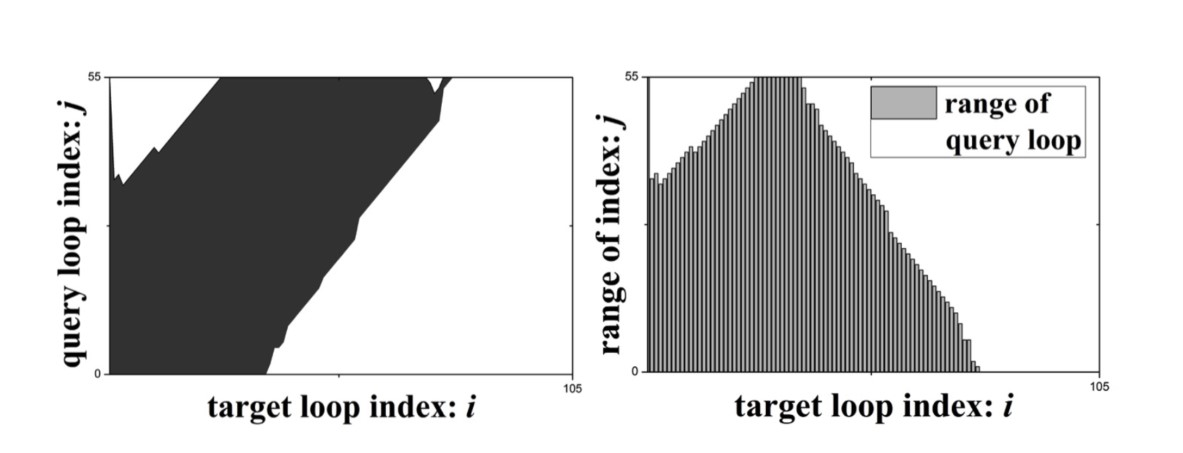
\includegraphics[width=0.9\linewidth]{banded}
    \caption{An example of BWA-MEM Smith-Waterman task. Left: cells actually computed in the matrix with pruning. Right: amount of elements calculated for each loop index. (from~\cite{Chen:acc})}
    \label{fig:banded}
\end{figure}{}
